\documentclass[crop=false]{standalone}

\usepackage[subpreambles=false]{standalone}
\usepackage{import}
\usepackage{graphicx}
\usepackage{subcaption}
\usepackage{tikz}

\begin{document}

\vspace{-0.015\linewidth}
\begin{center}
  % \hspace*{-0.08\linewidth}
  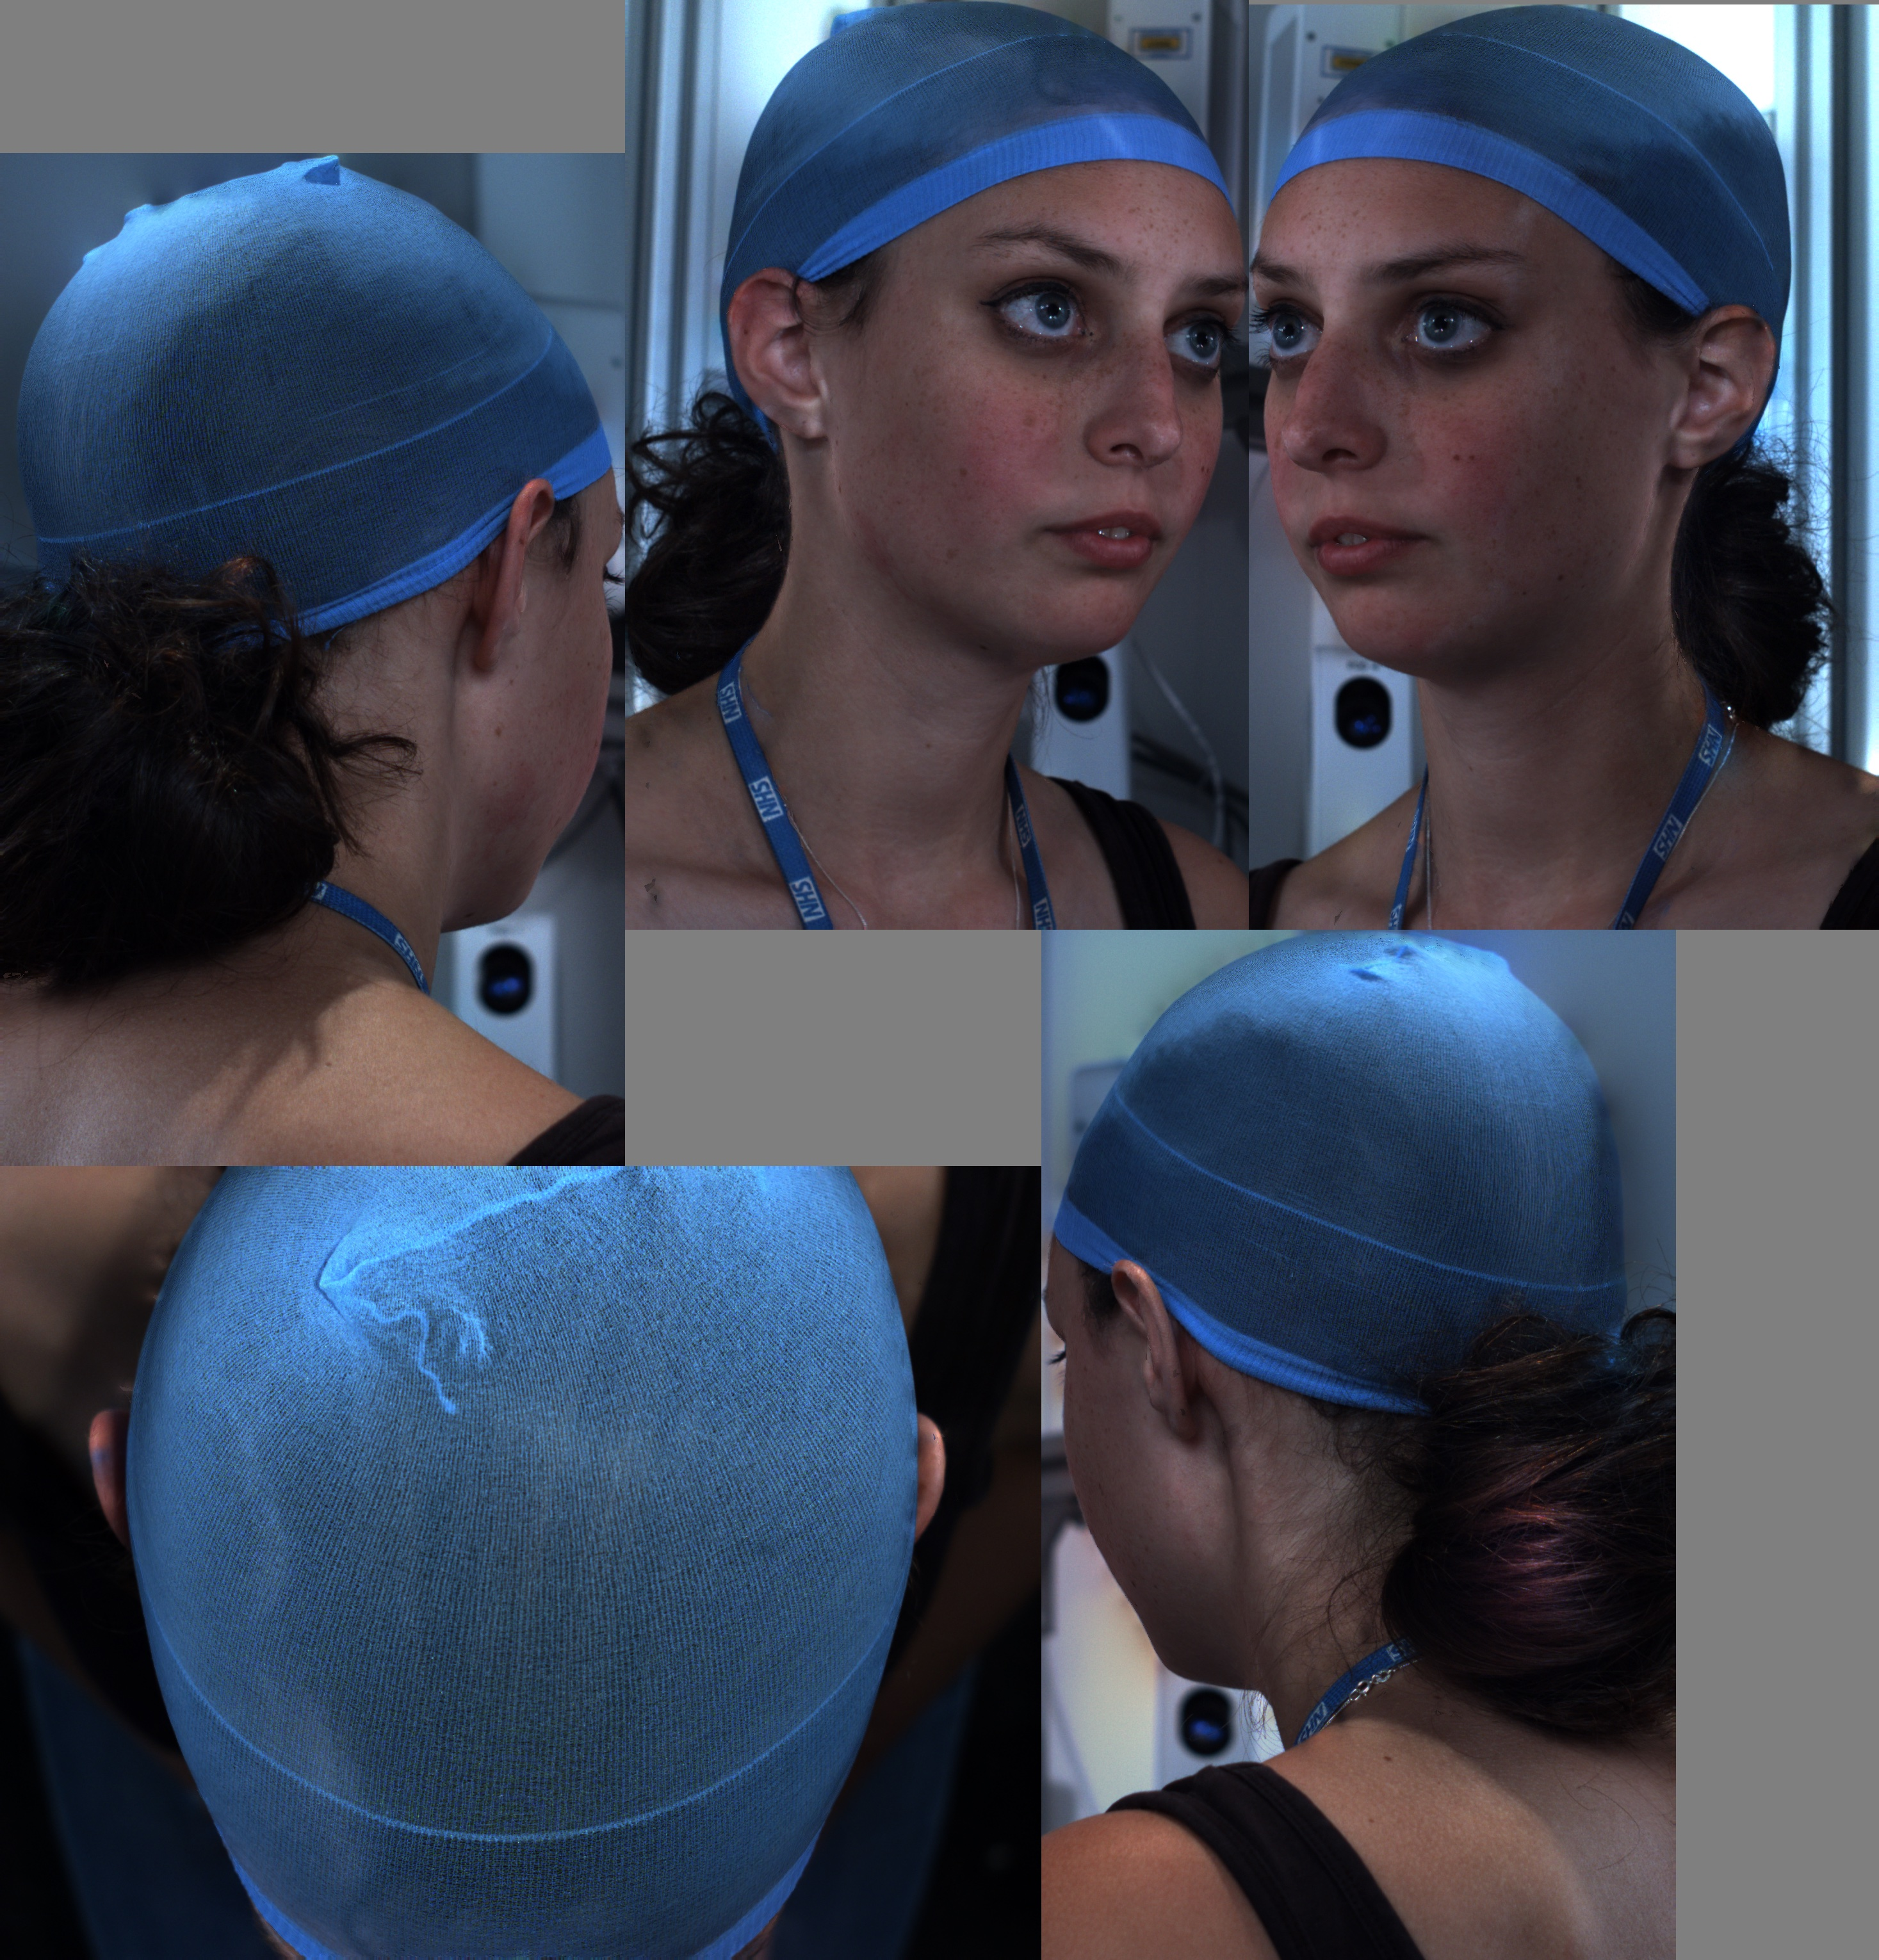
\includegraphics[width=0.7\linewidth]{thesis/imgs/stereophotogrammetry.jpg}
  %\vspace*{-0.06\linewidth}
  \captionof{figure}{
    \textbf{Stereophotogrammetry.}
    \small The patient is being photographed from 5 different angles around the head. Subsequently, the mesh is created by combining the different views into a single 3D mesh. Photo from Headspace dataset\cite{Dai2019}.
  }
  \label{fig:stereophotogrammetry}
\end{center}
\vspace{-0.01\linewidth}

\end{document}